% ****** Start of file aipsamp.tex ******
%
%   This file is part of the AIP files in the AIP distribution for REVTeX 4.
%   Version 4.1 of REVTeX, October 2009
%
%   Copyright (c) 2009 American Institute of Physics.

% Use this file as a source of example code for your aip document.
% Use the file aiptemplate.tex as a template for your document.
\documentclass[%
	aip,
	jmp,%
	amsmath,amssymb,
	%preprint,%
	reprint,%
	%author-year,%
	%author-numerical,%
]{revtex4-1}
\usepackage{graphicx}% Include figure files
\usepackage{grffile}
\usepackage{dcolumn}% Align table columns on decimal point
\usepackage{bm}% bold math
%\usepackage[mathlines]{lineno}% Enable numbering of text and display math
%\linenumbers\relax % Commence numbering lines
\usepackage{multirow}
\usepackage{color} % for the notes
\usepackage{etex}
\reserveinserts{58}
%\usepackage{morefloats}
\usepackage{hyperref}
\usepackage{xcolor}
\usepackage{amsmath}
\hypersetup{
	colorlinks,
	linkcolor={red!50!black},
	citecolor={blue!50!black},
	urlcolor={blue!80!black}
}

\usepackage{xr}
\externaldocument{supportingInformation}
\maxdeadcycles=1000

\usepackage{placeins}
\begin{document}

\preprint{XXXXX (preprint)}

%\title[Evolution of interaction networks]{On the evolution of interaction networks: primitive typology of vertex, prominence of measures and activity statistics}% Force line breaks with \\
%\title[Evolution of interaction networks]{On the evolution of interaction networks: a primitive typology of vertex}% Force line breaks with \\
%\title[Stability of interaction networks]{Stability in human interaction networks: sector relative sizes, prominence of topological measures and time activity statistics.}% Force line breaks with \\
%\title[Stability in human interaction networks]{Sector relative sizes and topological metrics time stability in human interaction networks}% Force line breaks with \\
\title[Interaction networks stability]{Time stability in human interaction networks}% Force line breaks with \\
\author{Renato Fabbri}%
\homepage{http://ifsc.usp.br/~fabbri/}
\email{fabbri@usp.br}
\affiliation{ 
	S\~ao Carlos Institute of Physics, University of S\~ao Paulo (IFSC/USP)%\\This line break forced with \textbackslash\textbackslash
}
%
%\author{Vilson V. da Silva Jr.}
%\homepage{http://automata.cc/}
%\email{vilson@void.cc}
%\altaffiliation[Also at ]{IFSC-USP}%Lines break automatically or can be forced with \\
%
%\author{Ricardo Fabbri}
%\homepage{http://www.lems.brown.edu/~rfabbri/}
%\email{rfabbri@iprj.uerj.br}
%\altaffiliation{
%	Instituto Polit\'ecnico, Universidade Estadual do Rio de Janeiro (IPRJ)
%}%Lines break automatically or can be forced with \\
%
%\author{Deborah C. Antunes}
%\homepage{http://lattes.cnpq.br/1065956470701739}
%\email{deborahantunes@gmail.com}
%\altaffiliation{
%	Curso de Psicologia, Universidade Federal do Cer\'a (UFC)
%}%Lines break automatically or can be forced with \\
%
%\author{Marilia M. Pisani}
%\homepage{http://lattes.cnpq.br/6738980149860322}
%\email{marilia.m.pisani@gmail.com}
%\altaffiliation{
	%Centro de Ciências Naturais e Humanas, Universidade Federal do ABC (CCNH/UFABC)
%}%Lines break automatically or can be forced with \\

%
%%\author{Luciano da Fontoura Costa}
%%  \homepage{http://cyvision.ifsc.usp.br/~luciano/}
%%  \email{ldfcosta@gmail.com}
%  \altaffiliation[Also at ]{IFSC-USP}%Lines break automatically or can be forced with \\

%\author{Osvaldo N. Oliveira Jr.}
%  \homepage{www.polimeros.ifsc.usp.br/professors/professor.php?id=4}
%  \email{chu@ifsc.usp.br}
% \altaffiliation[Also at ]{IFSC-USP}%Lines break automatically or can be forced with \\


\date{\today}% It is always \today, today,
%  but any date may be explicitly specified

\begin{abstract}
In this study, we demonstrate a remarkably stable activity in human interaction networks. The activity along time and topology evolution were investigated in four e-mail lists by considering window sizes from 50 to 10,000 messages, which were made to slide and generate snapshots of the network in a timeline. Furthermore, the activity in terms of seconds, minutes, hours, days and months, is practically the same for all lists. The activity of participants followed the expected scale-free behavior, thus allowing us to establish three classes of vertices by comparing with the Erd\"os-R\'enyi model, namely hubs, intermediary and peripheral vertices. The relative size of these three sectors did not vary with time and was essentially the same for all e-mail lists. Typically, 3-12\% of the vertices are hubs, 15-45\% are intermediary and the remainder are peripheral vertices. The metrics that contribute most to the dispersion of participants in the topological measures space were centrality measurements (degree, strength and betweenness), followed by symmetry-related metrics and then clustering coefficient. Similar results for the distribution of participants in the three categories and for the relative importance of the topological metrics were obtained for 12 additional networks from Facebook, Twitter and Participa.br. Consistent with expectations driven from the literature, these properties may be general for human interaction networks, which has important implications in establishing a typology based on objective, quantitative criteria.
\end{abstract}

\pacs{89.75.Fb,05.65.+b,89.65.-s}% PACS, the Physics and Astronomy
\keywords{complex networks, social network analysis, pattern recognition, statistics, anthropological physics}
\maketitle

\begin{quotation}
	`The reason for the persistent plausibility of the typological approach, however, is not a static biological one, but just the opposite: dynamic and social.' 
	% `The conception of personality structure is the
	%best safeguard against the
	% inclination to attribute persistent trends in the
	% individual to something
	% "innate" or "basic" or "racial" within him. The
	% Nazi allegation that natural, biological traits decide the total being of a % person
	% would not have been such
	% a successful political device
	% had it not been possible to point to numerous
	% instances of relative fixity in human behavior and to
	% challenge those who
	% thought to explain them on any basis other than a biological one.'
	\emph{- Adorno et al, 1969, p. 747}
\end{quotation}


\section{Introduction}\label{sec:into}
Studies on human interaction networks have started long before modern computers, dating back to the nineteenth century, while the foundation of
social network analysis is generally attributed to the psychiatrist Jacob Moreno in mid twentieth century~\cite{newmanBook}. With the increasing availability of data related to human interactions, research on these networks has grown continuously. Contributions can now be found in a variety of fields, from social sciences and humanities~\cite{latour2013} to computer science~\cite{bird} and physics~\cite{barabasiHumanDyn,newmanFriendship}, given the multidisciplinary nature of the topic. One of the approaches from an exact science perspective is to represent interaction networks as complex networks~\cite{barabasiHumanDyn,newmanFriendship}, with which 
several features of human interaction have been revealed. For example, the topology of human interaction networks exhibits a scale-free trace, which points to the existence of a small number of highly connected hubs and a large number of poorly connected nodes. The dynamics of complex networks representing human interaction has also been addressed ~\cite{barabasiEvo,newmanEvolving}, but only to a limited extent, since research is normally focused on a particular metric or task, such as accessibility or community detection~\cite{access,newmanModularity}. 

In this paper we analyze the evolution of human interaction networks, by considering interaction in email lists as their representative. Using a timeline of activity snapshots with a constant number of contiguous messages in email lists, we found a remarkable stability for several of the network properties. Because these properties were shared by networks from Twitter, Facebook and Participa.br, and are consistent with the literature, we advocate that some of the conclusions might be valid for more general classes of interaction networks. In particular, this allows us to discuss typologies in the context of such networks, in an attempt to bridge the gap between approaches based solely on data analysis (i.e. from a hard sciences perspective) and those relevant to the social sciences. This is important insofar as typologies are the canon of scientific literature for classification of human agents~\cite{typCanon}. 

The paper is organized as follows. Section~\ref{sec:related} describes related work, while details of the data and methods of analysis are given in  Section~\ref{sec:data} and Section~\ref{sec:carac}. Section~\ref{sec:results} brings the results and discussion, leading to Section~\ref{sec:conc} for conclusions. Details of how to access the data are given in the Appendix, while subsidiary results from the email lists and of networks from Twitter, Facebook and Participa.br are given in the Supporting Information.

\subsection{Related work}\label{sec:related}
Research on network evolution often considers solely network growth, in which there is a monotonic increase in the number of events considered~\cite{barabasiEvo}. Exceptions are reported in this section, with emphasis on those more closely related to the present article.

Network types have been discussed with regard to the number of participants, intermittence of their activity and network longevity~\cite{barabasiEvo}. Two topologically different networks emerged from human interaction networks, depending on the frequency of interactions, which can either be a generalized power law or an exponential connectivity distribution~\cite{barabasiTopologicalEv}. In email list networks, scale-free properties were reported with $\alpha=1$~\cite{bird} (as are web browsing and library loans~\cite{barabasiHumanDyn}), and different linguistic traces were related to weak and strong ties~\cite{GMANE2}.

Unreciprocated edges often exceed 50\% in the networks analyzed, which matches empirical evidence from the literature~\cite{newmanEvolving} and motivated the inclusion of symmetry metrics in our analysis. No correlation of topological characteristics and geographical coordinates was found~\cite{barabasiGeo}, therefore geographical positions were not considered in our study. Gender related behavior in mobile phone datasets was indeed reported~\cite{barabasiSex}, but this was not considered in the present article because email messages and addresses have no gender related metadata~\cite{gmanePack}.


\section{Data description: email lists and messages}\label{sec:data}

Email list messages were obtained from
the GMANE email archive~\cite{gmanePack}, which consists of more than 20,000 email lists and more than 130,000,000 messages~\cite{GMANEwikipedia}. These lists cover a variety of topics, mostly technology-related. The archive can be described as a corpus with metadata of its messages, including sent time, place, sender name, and sender email address.
The GMANE usage in scientific research is reported in studies of isolated lists and of lexical innovations~\cite{GMANE2,bird}. 

We analyzed many email lists (and data from Twitter, Facebook and Participa.br) but selected only four in order to make a thorough analysis, from which general properties can be inferred. These lists, selected as representing both a diverse set and ordinary lists, are:
\begin{itemize}
	\item Linux Audio Users list\footnote{gmane.linux.audio.users is list ID in GMANE.}, with participants holding hybrid artistic and technological interests, from different countries. English is the language used the most. Abbreviated as LAU from now on.
	\item Linux Audio Developers list\footnote{gmane.linux.audio.devel is list ID in GMANE.}, with participants from different countries, and English is the language used the most. A more technical and less active version of LAU. Abbreviated LAD from now on.
	\item Development list for the standard C++ library\footnote{gmane.comp.gcc.libstdc++.devel is list ID in GMANE.}, with computer programmers from different countries. English is the language used the most. Abbreviated as CPP from now on.
	\item List of the MetaReciclagem project\footnote{gmane.politics.organizations.metareciclagem is list ID in GMANE.}, with Brazilian activists holding digital culture interests. Portuguese is the most used language, although Spanish and English are also incident. Abbreviated MET from now on.
\end{itemize} 

The first 20,000 messages of each list were considered, with total timespan, authors, threads and missing messages indicated in Table~\ref{tab:genLists}.
In subsidiary experiments we considered 140 additional email lists, also retrieved from the GMANE public database, to analyze the interdependence between the number of participants and the number of threads. Furthermore, we used 12 additional networks from Facebook (8), Twitter (2) and Participa.br (2) to grasp the generality of the results driven from email lists.

\begin{table}
	\centering
	\caption{Columns $date_1$ and $date_M$ have dates of first and last messages from the 20,000 messages considered in each email list.
		$N$ is the number of participants (number of different email addresses).
		$\Gamma$ is the number of threads (count of messages without antecedent).
		$\overline{M}$ is the number of messages missing in the 20,000 collection, $100\frac{23}{20000}=0.115$ percent in the worst case.
	A relation holds for all these lists: within a same number of messages, as the number of participants increases, the number of threads decreases.}
	\label{tab:genLists}
	\begin{tabular}{|l|c|c|c|c|c|}\hline
		list & $date_1$ & $date_{M}$    & $N$  & $\Gamma$ & $\overline{M}$ \\\hline
		LAU & 2003-06-29  & 2005-07-23  & 1181  & 3372  & 5 \\\hline
LAD & 2003-06-30  & 2009-10-07  & 1268  & 3109  & 4 \\\hline
MET & 2005-08-01  & 2008-03-07  & 492  & 4607  & 23 \\\hline
CPP & 2002-03-12  & 2009-08-25  & 1052  & 4506  & 7 \\\hline

	\end{tabular}
\end{table}


\section{Characterization methods}\label{sec:carac}
The email lists and the networks generated from them were characterized using five procedures, namely: 1) statistics of activity along time, in scales from seconds to years; 2) sectioning of the networks in hubs, intermediary and peripheral vertices; 3) dispersion of basic topological metrics; 4) iterative visualization and data inspection.
Each of these procedures are described below.

\subsection{Time activity statistics}\label{sec:mtime}
Messages were counted along time with respect to seconds, minutes, hours, days of the week, days of the month, and months of the year. This resulted in histograms from which patterns could be drawn. The ratio $\frac{b_h}{b_l}$ between the highest and lowest incidences on the histograms served as a hint of how close the observed distribution is to a uniform distribution.

The average and the dispersion were taken using circular statistics, in which each $measurement$ (data point) is represented as a complex number with modulus equal to one, $z=e^{i\theta}=\cos(\theta)+i\sin(\theta)$, where $\theta=measurement\frac{2\pi}{period}$. The moments $m_n$, lengths of moments $R_n$, mean angle $\theta_\mu$, and rescaled mean angle $\theta_\mu'$ are defined as:

\begin{align}\label{eq:cmom}
	m_n&=\frac{1}{N}\sum_{i=1}^N z_i^n \nonumber\\
	R_n&=|m_n|\\
	\theta_\mu&=Arg(m_1) \nonumber \\
	\theta_\mu'&=\frac{period}{2\pi} \theta_\mu \nonumber
\end{align}

$\theta_\mu'$ is used as the measure of location. Dispersion is measured using the circular variance $Var(z)$, the circular standard deviation $S(z)$, and the circular dispersion $\delta(z)$:

\begin{align}\label{eq:cmd}
	Var(z)&=1 - R_1 \nonumber\\
	S(z)&= \sqrt{-2\ln(R_1)}\\
	\delta(z)&=\frac{1-R_2}{2 R_1^2} \nonumber
\end{align}

As expected, a positive correlation was found in all $Var(z)$, $S(z)$ and $\delta(z)$ dispersion measures, as can be noticed in Section~\ref{si:circ} of the Supporting Information, and $\delta(z)$ was preferred in the discussion of results.

\subsection{Interaction networks}\label{intNet}
Interaction networks can be modeled both weighted or unweighted, both directed or undirected~\cite{bird,newmanCommunityDirected,newmanCommunity2013}.
Networks in this article are directed and weighted, the more informative of trivial possibilities, i.e. we did not investigate directed unweighted, undirected weighted, and undirected unweighted representations of the interaction networks. 
The networks were obtained as follows: a direct response from participant B to a message from participant A yields an edge from A to B, as information went from A to B. The reasoning is: if B wrote a response to a message from A, he/she read what A wrote and formulated a response, so B assimilated information from A, thus $A \rightarrow B$. Inverting edge direction yields the status network: B read the message and considered what A wrote worth responding, giving status to A, thus $B\rightarrow A$. This article uses the information network as described above and depicted in Figure~\ref{formationNetwork}. Edges in both directions are allowed. Each time an interaction occurs, one is added to the edge weight. Selfloops were regarded as non-informative and discarded. These human social interaction networks are reported in the literature as exhibiting scale-free and small world properties, as expected for (some) social networks~\cite{bird,newmanBook}.

\begin{figure}[!h]
	\centering
	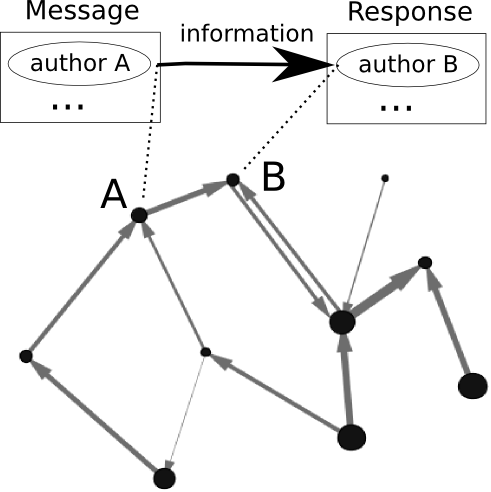
\includegraphics[width=0.5\textwidth]{figs/criaRede__}
	\caption{Formation of interaction network from email messages. Each vertex represents a participant. A reply message from participant B to a message from participant A is regarded as evidence that B received information from A and yields a directed edge. Multiple messages add ``weight'' to a directed edge. Further details are given in Section~\ref{intNet}.}
	\label{formationNetwork}
\end{figure}

Edges can be created from all antecedent message authors on the message-response thread to each message author.
We only linked the immediate antecedent to the new message author, both for simplicity and for the valid objection that in adding two edges, $x\rightarrow y$ and $y\rightarrow z$, there is also a weaker connection between $x$ and $z$. Potential interpretations for this weaker connection are: double length, half weight or with one more ``obstacles''. This suggests the adequacy of centrality measurements to account for the connectivity with all nodes, such as betweenness centrality, eigenvector centrality and accessibility~\cite{luMeasures,access}.

%\subsubsection{Sectioning of networks in peripheral, intermediary and hubs sectors}\label{sectioning}
\subsection{Erd\"os sectioning}\label{sectioning}
In a scale-free network, the peripheral, intermediary and hubs sectors can be derived from a comparison with an Erd\"os-R\'enyi network with the same number of edges and vertices~\cite{3setores}, as depicted in Figure~\ref{fig:setores}. We shall refer to this procedure as \emph{Erd\"os sectioning}, with the resulting sectors being referred to as \emph{Erd\"os sectors} or \emph{primitive sectors}.

The degree distribution $\widetilde{P}(k)$ of an ideal
scale-free network $\mathcal{N}_f$ with $N$ vertices and $z$ edges has less
average degree nodes than the distribution $P(k)$ of an Erd\"os-R\'enyi
network with the same number of vertices and edges. Indeed, we define in this work the intermediary sector of a network to be the set of all the nodes whose degree is less abundant in the real network than on the Erd\"os-R\'enyi model:

\begin{equation}\label{criterio}
	\widetilde{P}(k)<P(k) \Rightarrow \text{k is intermediary degree}
\end{equation}

If $\mathcal{N}_f$ is directed and has no self-loops, the probability
of an edge between two arbitrary vertices is $p_e=\frac{z}{N(N-1)}$.
A vertex in the ideal Erd\"os-R\'enyi digraph with the same number of vertices and edges, and thus the same probability $p_e$ for the presence of an edge, will have degree $k$ with probability:

\begin{equation}
	P(k)=\binom{2(N-1)}{k}p_e^k(1-p_e)^{2(N-1)-k}
\end{equation}

The lower degree fat tail consists on the border vertices, i.e. the peripheral sector or periphery where $\widetilde{P}(k)>P(k)$ and $k$ is lower than any intermediary sector value of $k$. The higher degree fat tail is the hub sector, i.e. $\widetilde{P}(k)>P(k)$ and $k$ is higher than any intermediary sector value of $k$. The reasoning for this classification is: vertices so connected that they are virtually inexistent in networks connected at pure chance (e.g. without preferential attachment) are correctly associated to the hubs sector. Vertices with very few connections, which are way more abundant than expected by pure chance, are assigned to the periphery. Vertices with degree values predicted as the most abundant if connections are created by pure chance, near the average, and less frequent in the real network, are classified as intermediary.

\begin{figure}[!h]
	\centering
	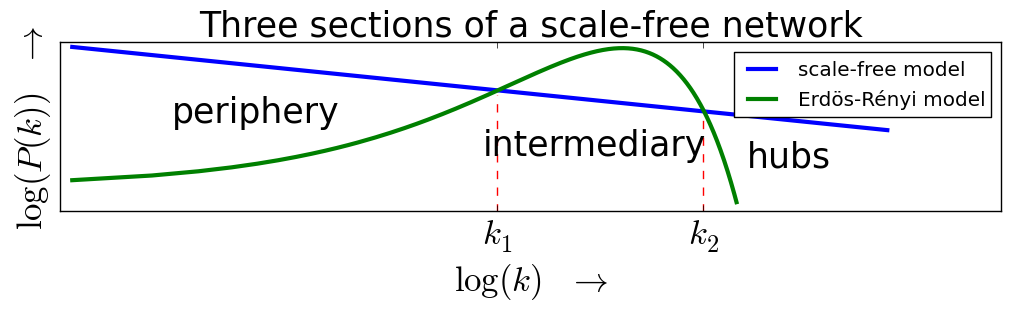
\includegraphics[width=0.5\textwidth]{figs/fser_}
	\caption{Degree distribution of scale-free and Erd\"os-R\'enyi ideal networks.
		The latter has more intermediary vertices, while the former has more peripheral and hub vertices.
		The sector borders are defined by the two intersections $k_L$ and $k_R$ of the connectivity distributions.
		Characteristic degrees are in the compact intervals: $[0,k_L]$, $(k_L,k_R]$, $(k_R,k_{max}]$ for the Erd\"os sectors (periphery, intermediary and hubs).}
		\label{fig:setores}
\end{figure}
i	To ensure statistical validity of the histograms, bins can be chosen to contain at least $\eta$ vertices of the real network. Thus, each bin, starting at degree $k_i$, spans $\Delta_i=[k_{i},k_{j}]$ degree values, where $j$ is the smallest integer with which there are at least $\eta$ vertices with degree larger than or equal $k_i$, and less than or equal $k_{j}$. This changes equation~\ref{criterio} to:

\begin{equation}\label{criterio2}
	\sum_{x=k_i}^{k_j} \widetilde{P}(x) < \sum_{x=k_i}^{k_j} P(x) \Rightarrow \text{i is intermediary}
\end{equation}

If strength $s$ is used for comparison, $P$ remains the same, but $P(\kappa_i)$ with $\kappa_i=\frac{s_i}{\overline{w}}$ should be used for comparison, with $\overline{w}=2\frac{z}{\sum_is_i}$ the average weight of an edge and $s_i$ the strength of vertex $i$. For in and out degrees ($k^{in}$, $k^{out}$) comparison of the real network should be made with:
\begin{equation}
	\hat{P}(k^{way})=\binom{N-1}{k^{way}}p_e^k(1-p_e)^{N-1-k^{way}}
\end{equation}

\noindent where \emph{way} can be \emph{in} or \emph{out}. In and out strengths ($s^{in}$, $s^{out}$) are divided by $\overline{w}$ and compared also using $\hat{P}$. Note that $p_e$ remains the same, as each edge yields an incoming (or outgoing) edge, and there are at most $N(N-1)$ incoming (or outgoing) edges, thus $p_e=\frac{z}{N(N-1)}$ as with the total degree.

In other words, let $\gamma$ and $\phi$ be integers in the intervals $1 \leq \gamma \leq 6$, $1 \leq \phi \leq 3$, and each of the basic six Erd\"os sectioning possibilities $\{E_{\gamma}\}$ have three Erd\"os sectors $E_{\gamma}= \{e_{\gamma, \phi} \}$ defined as:

\begin{alignat}{3}\label{eq:part}
	e_{\gamma,1}&=\{\;i\;|\;\overline{k}_{\gamma,L}\geq&&\overline{k}_{\gamma,i}\} \nonumber \\
	e_{\gamma,2}&=\{\;i\;|\;\overline{k}_{\gamma,L}<\;&&\overline{k}_{\gamma,i}\leq\overline{k}_{\gamma,R}\} \\ 
	e_{\gamma,3}&=\{\;i\;|\;&&\overline{k}_{\gamma,i}<\overline{k}_{\gamma,R}\} \nonumber
\end{alignat}

\noindent where $\{\overline{k}_{\gamma,i}\}$ is:

\begin{equation}
	\begin{split}
		\overline{k}_{1,i}&=k_i \\
		\overline{k}_{2,i}&=k_i^{in} \\
		\overline{k}_{3,i}&=k_i^{out} \\
		\overline{k}_{4,i}&=\frac{s_i}{\overline{w}} \\
		\overline{k}_{5,i}&=\frac{s_i^{in}}{\overline{w}} \\
		\overline{k}_{6,i}&=\frac{s_i^{out}}{\overline{w}} \\
	\end{split}
\end{equation}

\noindent and both $\overline{k}_{\gamma,L}$ and $\overline{k}_{\gamma,R}$ are found using $P(\overline{k})$ or $\hat{P}(\overline{k})$ as described above.

Since different metrics can be used to identify the three types of vertices, compound criteria can be defined. For example, a very stringent criterion can be used, according to which a vertex is only regarded as pertaining to a sector if it is so for all the metrics. After a careful consideration of possible combinations, these were reduced to six:

\begin{itemize}
	\item Exclusivist criterion $C_1$:  vertices are only classified if the class is the same according to all metrics. In this case, vertices classified (usually) do not reach 100\%, which is indicated by a black line in Figure~\ref{fig:sectIL}.
	\item Inclusivist criterion $C_2$: a vertex has the class given by any of the metrics. Therefore, a vertex may belong to more than one class, and the total number of members may exceed 100\%, which is indicated by a black line in Figure~\ref{fig:sectIL}.
	\item Exclusivist cascade $C_3$: vertices are only classified as hubs if they are hubs according to all metrics. Intermediary are the vertices classified either as intermediary or hubs with respect to all metrics. The remaining vertices are regarded as peripheral.
	\item Inclusivist cascade $C_4$: vertices are hubs if they are classified as so according to any of the metrics. The remaining vertices are classified as intermediary if they belong to this category for any of the metrics. Peripheral vertices will then be those which were not classified as hub or intermediary with any of the metrics. 
	\item Exclusivist externals $C_5$: vertices are only hubs if they are classified as such according to all the metrics. The remaining vertices are classified as peripheral if they fall into the periphery or hub classes by any metric. The rest of the nodes are classified as intermediary.
	\item Inclusivist externals $C_6$: hubs are vertices classified as hubs according to any metric. The remaining vertices will be peripheral if they are classified as such according to any metric. The rest of the vertices will be intermediary vertices.
\end{itemize}

Using equations~\ref{eq:part}, these compound criteria $C_\delta$, with $\delta$ integer in the interval $1<\delta<6$ can be described as:

%\begin{alignat}{3}
\begin{equation}
	\begin{split}
		%\begin{multline}
		C_1&=\{c_{1,\phi}=\left\{i\mid i\;\in e_{\gamma,\phi}, \;\forall\; \gamma\}\right\} \\
		C_2&=\{c_{2,\phi}=\left\{i\mid \exists \;\;\gamma: i \in e_{\gamma,\phi}\}\right\} \\
		C_3&=\{c_{3,\phi}=\left\{i\mid i\;\in e_{\gamma,\phi'}, \;\forall\; \gamma,\;\forall\;\phi'\geq \phi\}\right\} \\
		C_4&=\{c_{4,\phi}=\left\{i\mid i\;\in e_{\gamma,\phi'}, \;\forall\; \gamma,\;\forall\;\phi'\leq \phi\}\right\} \\
		C_5&=\{c_{5,\phi}=\left\{i\mid i\;\in e_{\gamma,\phi'}, \;\forall\; \gamma,\right.\\
																																	&\;\;\;\;\;\;\;\;\;\;\;\;\;\;\;\;\;\; \left.\;\forall\;(\phi'+1)\%4\leq (\phi+1)\%4\}\right\} \\
		C_6&=\{c_{6,\phi}=\left\{i\mid i\;\in e_{\gamma,\phi'}, \;\forall\; \gamma,\right.\\
																																	&\;\;\;\;\;\;\;\;\;\;\;\;\;\;\;\;\;\; \left.\;\forall\;(\phi'+1)\%4\geq (\phi+1)\%4\}\right\} \\
		%\end{multline}
	\end{split}
\end{equation}
%\end{alignat}

The simplification of all the compound possibilities to the small set listed above can be formalized in strict mathematical terms, but this was considered out of the scope for current interests. It is worth noting that the exclusivist cascade is the same sectioning of an inclusivist cascade from periphery to hubs, but with inverted order of sectors precedence. These compound criteria can be used to examine network sections considering all degrees and strengths and are specially useful in the case of a low number of messages, such as in Section~\ref{si:frac} of the Supporting Information.

\subsection{Topological metrics for Principal Component Analysis}\label{measures}

The topology of the networks was studied using Principal Component Analysis (PCA~\cite{pca}) with a small selection of the most basic and fundamental measurements for each vertex, as follows:

\begin{itemize}
	\item Degree     $k_i$: number of edges linked to vertex $i$.
	\item In-degree  $k_i^{in}$: number of edges ending at vertex $i$.
	\item Out-degree $k_i^{out}$: number of edges departing from vertex $i$.
	\item Strength $s$: sum of weights of all edges linked to vertex $i$.
	\item In-strength $s_i^{in}$: sum of weights of all edges ending at vertex $i$.
	\item Out-strength $s_i^{out}$: sum of weights of all edges departing from vertex $i$.
	\item Clustering coefficient $cc_i$: fraction of pairs of neighbors of $i$ that are linked.  The standard clustering coefficient for undirected graphs was used.
	\item Betweenness centrality $bt_i$: fraction of geodesics that contain vertex $i$. The betweenness centrality index considered directions and weight, as specified in~\cite{faster}.
\end{itemize}

In order to capture symmetries in the activity of participants, the following metrics were introduced for a vertex $i$: 

\begin{itemize}
	\item Asymmetry: $asy_i=\frac{k_i^{in}-k_i^{out}}{k_i}$.
	\item Mean of asymmetry of edges: $\mu_i^{asy}=\frac{\sum_{j\in J_i} e_{ji}-e_{ij}}{|J_i|=k_i}$, where $e_{xy}$ is 1 if there is an edge from $x$ to $y$, and $0$ otherwise. $J_i$ is the set of neighbors of vertex $i$, and $|J_i|=k_i$ is the number of neighbors of vertex $i$.
	\item Standard deviation of asymmetry of edges: $\sigma_i^{asy}=\sqrt{\frac{\sum_{j\in J_i}[\mu_{asy} -(e_{ji}-e_{ij}) ]^2  }{k_i}  }$.
	\item Disequilibrium: $dis_i=\frac{s_i^{in}-s_i^{out}}{s_i}$.
	\item Mean of disequilibrium of edges: $\mu_i^{dis}=\frac{\sum_{j \in J_i}\frac{w_{ji}-w_{ij}}{s_i}}{k_i}$, where $w_{xy}$ is the weight of edge $x\rightarrow y$ and zero if there is no such edge.
	\item Standard deviation of disequilibrium of edges: $\sigma_i^{dis}=\sqrt{\frac{\sum_{j\in J_i}[\mu_{dis}-\frac{(w_{ji}-w_{ij})}{s_i}]^2}{k_i}}$.
\end{itemize}

\subsection{Evolution and visualization of the networks}\label{sec:viz}
The evolution of the networks was observed within a fixed number of messages, which we refer to as the window size $ws$. This same number of contiguous messages $ws$ was considered with different shifts in the message timeline to obtain snapshots. Each snapshot was used both to perform the Erd\"os sectioning and to apply PCA for the topological metrics.  
The $ws$ used were 50, 100, 200, 400, 500, 800, 1000, 2000, 2500, 5000 and 10000. Within a same $ws$, the number of vertices and edges vary in time, as do other network characteristics, which is exhibited in Section~\ref{si:frac} of the Supporting Information. 

Networks were visualized with animations, image galleries and online gadgets developed specifically for this research~\cite{animacoes,galGMANE,appGMANE}. Such visualizations were crucial to guide research into the most important features of network evolution. Furthermore, the size of the three Erd\"os sectors could be visualized in a timeline fashion. Visualization of network structure was especially useful in the inspection of data and derived structures from the email lists.

\section{Results and discussion}\label{sec:results}
%Remarkable features from the analysis of the four email lists are:
%\begin{itemize}
%    \item The activity along time is practically the same for all lists, thus suggesting stable patterns.
%    \item The fraction of participants in each Erd\"os sector is stable along time and can be determined even with very few messages 
%    \item The topological metrics combine into principal components in PCA in the same way for all lists and all snapshots (). 
%        \item Symmetry measures of the topology, as defined in this article, present more dispersion than the usual clustering coefficient (Section~\ref{prevalence}).
%    \item Typology speculations are immediate from results (Section~\ref{sec:pty}).
%\end{itemize}
\subsection{Activity along time}\label{constDisc}
The activity along time, in terms of seconds, minutes, hours, days and months,  is practically the same for all lists.
Histograms in each time scale were calculated as were circular average values and their dispersion.
We chose to give detailed values in Table~\ref{tab:circ}-\ref{tab:min2} because these numbers can actually be used for characterizing nodes (participants) in other networks, and networks themselves, as they are independent of the network under analysis. For example, they may serve for identification of outliers in a community.

\begin{table}
	\caption{The rescaled circular mean $\theta_\mu'$ and the circular dispersion $\delta(z)$ described in Section~\ref{sec:mtime}.
		This typical table was made using all LAD list messages, and the results are the same for other lists, as shown in Section~\ref{si:circ} of the Supporting Information.
	Most uniform distribution of activity was found in seconds and minutes, where the mean has little meaning.
	Hours of the day exhibited the most concentrated activity (lowest $\delta(z)$), with mean between 14h and 15h ($\theta'=-9.61$).
	Weekdays, month days and months have mean near zero (i.e. near the beginning of the week, month and year) and high dispersion.}
	\begin{center}
		\begin{tabular}{ |l|| c|c| }
			\hline
			%scale & $\theta_\mu'$ & $S(z)$ & $Var(z)$ & $\delta(z)$ & $\frac{max(incidence)}{min(incidence)}$ & $ \mu_{\frac{max(incidence')}{min(incidence')}} $ & $ \sigma_{\frac{max(incidence')}{min(incidence')} } $ \\ \hline\hline
			%& $\theta_\mu'$ & $S(z)$ & $Var(z)$ & $\delta(z)$  \\ \hline\hline
			& $\theta_\mu'$ & $\delta(z)$  \\ \hline\hline
			seconds    & --//--  & 9070.17     \\\hline
minutes    & --//--  & 205489.40   \\\hline
hours      & -9.61   & 4.36        \\\hline
weekdays   & -0.03   & 29.28       \\\hline
month days & -2.65   & 2657.77     \\\hline
months     & -0.56   & 44.00       \\\hline

		\end{tabular}
	\end{center}
	\label{tab:circ}
\end{table}

\begin{table}
	\caption{Activity percentages along the hours of the day for the CPP list. Nearly identical distributions are found on other lists as shown in Section~\ref{si:hours} of the Supporting Information. Higher activity was observed between noon and 6pm, followed by the time period between 6pm and midnight. Around 2/3 of the whole activity takes place from noon to midnight. Nevertheless, the activity peak occurs around midday, with a slight skew toward one hour before noon.}
	\footnotesize
	\begin{center} 
 \begin{tabular}{| l || c | c | c | c | c | c |}\hline 
  & 1h & 2h & 3h & 4h & 6h & 12h \\\hline 
 0h  &  \multirow{1}{*}{ 3.66 }   &  \multirow{2}{*}{ 6.42 }   &  \multirow{3}{*}{ 8.20 }   &  \multirow{4}{*}{ 9.30 }   &  \multirow{6}{*}{ 10.67 }   &  \multirow{12}{*}{ 33.76 }  \\\cline{2-2} 
 1h  &  \multirow{1}{*}{ 2.76 }   &   &   &   &   &  \\\cline{2-2}\cline{3-3} 
 2h  &  \multirow{1}{*}{ 1.79 }   &  \multirow{2}{*}{ 2.88 }   &   &   &   &  \\\cline{2-2}\cline{4-4} 
 3h  &  \multirow{1}{*}{ 1.10 }   &   &  \multirow{3}{*}{ 2.47 }   &   &   &  \\\cline{2-2}\cline{3-3}\cline{5-5} 
 4h  &  \multirow{1}{*}{ 0.68 }   &  \multirow{2}{*}{ 1.37 }   &   &  \multirow{4}{*}{ 3.44 }   &   &  \\\cline{2-2} 
 5h  &  \multirow{1}{*}{ 0.69 }   &   &   &   &   &  \\\cline{2-2}\cline{3-3}\cline{4-4}\cline{6-6} 
 6h  &  \multirow{1}{*}{ 0.83 }   &  \multirow{2}{*}{ 2.07 }   &  \multirow{3}{*}{ 4.35 }   &   &  \multirow{6}{*}{ 23.09 }   &  \\\cline{2-2} 
 7h  &  \multirow{1}{*}{ 1.24 }   &   &   &   &   &  \\\cline{2-2}\cline{3-3}\cline{5-5} 
 8h  &  \multirow{1}{*}{ 2.28 }   &  \multirow{2}{*}{ 6.80 }   &   &  \multirow{4}{*}{ 21.03 }   &   &  \\\cline{2-2}\cline{4-4} 
 9h  &  \multirow{1}{*}{ 4.52 }   &   &  \multirow{3}{*}{ 18.75 }   &   &   &  \\\cline{2-2}\cline{3-3} 
 10h  &  \multirow{1}{*}{ 6.62 }   &  \multirow{2}{*}{ \textbf{ 14.23 } }   &   &   &   &  \\\cline{2-2} 
 11h  &  \multirow{1}{*}{ \textbf{ 7.61 } }   &   &   &   &   &  \\\cline{2-2}\cline{3-3}\cline{4-4}\cline{5-5}\cline{6-6}\cline{7-7} 
 12h  &  \multirow{1}{*}{ 6.44 }   &  \multirow{2}{*}{ 12.48 }   &  \multirow{3}{*}{ \textbf{ 18.95 } }   &  \multirow{4}{*}{ \textbf{ 25.05 } }   &  \multirow{6}{*}{ \textbf{ 37.63 } }   &  \multirow{12}{*}{ \textbf{ 66.24 } }  \\\cline{2-2} 
 13h  &  \multirow{1}{*}{ 6.04 }   &   &   &   &   &  \\\cline{2-2}\cline{3-3} 
 14h  &  \multirow{1}{*}{ 6.47 }   &  \multirow{2}{*}{ 12.57 }   &   &   &   &  \\\cline{2-2}\cline{4-4} 
 15h  &  \multirow{1}{*}{ 6.10 }   &   &  \multirow{3}{*}{ 18.68 }   &   &   &  \\\cline{2-2}\cline{3-3}\cline{5-5} 
 16h  &  \multirow{1}{*}{ 6.22 }   &  \multirow{2}{*}{ 12.58 }   &   &  \multirow{4}{*}{ 23.60 }   &   &  \\\cline{2-2} 
 17h  &  \multirow{1}{*}{ 6.36 }   &   &   &   &   &  \\\cline{2-2}\cline{3-3}\cline{4-4}\cline{6-6} 
 18h  &  \multirow{1}{*}{ 6.01 }   &  \multirow{2}{*}{ 11.02 }   &  \multirow{3}{*}{ 15.88 }   &   &  \multirow{6}{*}{ 28.61 }   &  \\\cline{2-2} 
 19h  &  \multirow{1}{*}{ 5.02 }   &   &   &   &   &  \\\cline{2-2}\cline{3-3}\cline{5-5} 
 20h  &  \multirow{1}{*}{ 4.85 }   &  \multirow{2}{*}{ 9.23 }   &   &  \multirow{4}{*}{ 17.59 }   &   &  \\\cline{2-2}\cline{4-4} 
 21h  &  \multirow{1}{*}{ 4.38 }   &   &  \multirow{3}{*}{ 12.73 }   &   &   &  \\\cline{2-2}\cline{3-3} 
 22h  &  \multirow{1}{*}{ 4.06 }   &  \multirow{2}{*}{ 8.36 }   &   &   &   &  \\\cline{2-2} 
 23h & \multirow{1}{*}{ 4.30 }  & & & & & \\\cline{2-2}\cline{3-3}\cline{4-4}\cline{5-5}\cline{6-6}\cline{7-7} 
 \hline\end{tabular} 
 \end{center}
	\label{tab:hin}
\end{table}


\begin{table}
	\caption{Activity percentages along the days of the week for the four email lists. Higher activity was observed during weekdays, with a decrease of activity on weekends of at least one third and two thirds in extreme cases.}
	\begin{center}
		\begin{tabular}{ | l |  c | c | c | c | c |   c | c |}
			\hline
			& Mon & Tue & Wed & Thu & Fri & Sat & Sun  \\ \hline
			LAU & 15.71  & 15.81  & 15.88  & 16.43  & 15.14  & {\bf 10.13}  & {\bf 10.91} \\\hline
LAD & 14.92  & 17.75  & 17.01  & 15.41  & 14.21  & {\bf 10.40}  & {\bf 10.31} \\\hline
MET & 17.53  & 17.54  & 16.43  & 17.06  & 17.46  & {\bf 7.92 }  & {\bf 6.06 }\\\hline
CPP & 17.06  & 17.43  & 17.61  & 17.13  & 16.30  & {\bf 6.81 }  & {\bf 7.67 }\\\hline

		\end{tabular}
	\end{center}
	\label{tab:win}
\end{table}
In the scale of seconds and minutes, activity obeys a homogeneous pattern, with the messages being slightly more evenly distributed in all lists than in simulations using uniform distribution\footnote{Numpy version 1.6.1, ``random.randint'' function, was used for simulations, algorithms in \url{https://pypi.python.org/pypi/gmane}.}. In the networks, $\frac{max(incidence)}{min(incidence)} \in (1.26,1.275]$ while simulations reach these values but have in average more discrepant higher and lower peaks $\xi=\frac{max(incidence')}{min(incidence')} \Rightarrow \mu_\xi=1.2918 \text{ and } \sigma_\xi=0.04619$.
Therefore, the incidence of messages at each second of a minute and at each minute of an hour was considered uniform, i.e. no trend was detected. Circular dispersion is maximized and the mean has little meaning as indicated in Table~\ref{tab:circ}. As for the hours of the day, an abrupt peak appeared around 11am with the most active period being the afternoon. Days of the week revealed a decrease of at least one third and at most two thirds of activity on weekends. Days of the month were regarded as homogeneous with an inconclusive slight tendency of the first week being more active. Months of the year revealed patterns matching usual work and academic calendars. The time period examined here was not sufficient for the analysis of activity along the years. These patterns are exemplified in Tables~\ref{tab:hin}-\ref{tab:min2}.


\FloatBarrier

\begin{table}
	\caption{Activity in the days along the month for MET list. Nearly identical distributions are found on other lists as indicated in Section~\ref{si:monthdays} of the Supporting Information. Although slightly higher activity rates are found in the beginning of the month, the most important feature seems to be the homogeneity made explicit by the high circular dispersion in Table~\ref{tab:circ}.}
	\footnotesize
	\begin{center}
\begin{tabular}{| l || c | c | c | c |}\hline
 & 1 day & 5 & 10 & 15 days \\\hline
1 & \multirow{1}{*}{ 3.05 }  & \multirow{5}{*}{ 18.25 }  & \multirow{10}{*}{ 35.24 }  & \multirow{15}{*}{ 50.96 }  \\\cline{2-2}
2 & \multirow{1}{*}{ 3.38 }  & & & \\\cline{2-2}
3 & \multirow{1}{*}{ 3.62 }  & & & \\\cline{2-2}
4 & \multirow{1}{*}{ 4.25 }  & & & \\\cline{2-2}
5 & \multirow{1}{*}{ 3.94 }  & & & \\\cline{2-2}\cline{3-3}
6 & \multirow{1}{*}{ 3.73 }  & \multirow{5}{*}{ 16.98 }  & & \\\cline{2-2}
7 & \multirow{1}{*}{ 3.17 }  & & & \\\cline{2-2}
8 & \multirow{1}{*}{ 3.26 }  & & & \\\cline{2-2}
9 & \multirow{1}{*}{ 3.56 }  & & & \\\cline{2-2}
10 & \multirow{1}{*}{ 3.26 }  & & & \\\cline{2-2}\cline{3-3}\cline{4-4}
11 & \multirow{1}{*}{ 3.81 }  & \multirow{5}{*}{ 15.73 }  & \multirow{10}{*}{ 31.98 }  & \\\cline{2-2}
12 & \multirow{1}{*}{ 2.91 }  & & & \\\cline{2-2}
13 & \multirow{1}{*}{ 3.30 }  & & & \\\cline{2-2}
14 & \multirow{1}{*}{ 2.75 }  & & & \\\cline{2-2}
15 & \multirow{1}{*}{ 2.95 }  & & & \\\cline{2-2}\cline{3-3}\cline{5-5}
16 & \multirow{1}{*}{ 3.36 }  & \multirow{5}{*}{ 16.25 }  & & \multirow{15}{*}{ 49.04 }  \\\cline{2-2}
17 & \multirow{1}{*}{ 3.16 }  & & & \\\cline{2-2}
18 & \multirow{1}{*}{ 3.44 }  & & & \\\cline{2-2}
19 & \multirow{1}{*}{ 3.36 }  & & & \\\cline{2-2}
20 & \multirow{1}{*}{ 2.93 }  & & & \\\cline{2-2}\cline{3-3}\cline{4-4}
21 & \multirow{1}{*}{ 3.20 }  & \multirow{5}{*}{ 15.79 }  & \multirow{10}{*}{ 32.78 }  & \\\cline{2-2}
22 & \multirow{1}{*}{ 3.11 }  & & & \\\cline{2-2}
23 & \multirow{1}{*}{ 3.60 }  & & & \\\cline{2-2}
24 & \multirow{1}{*}{ 2.74 }  & & & \\\cline{2-2}
25 & \multirow{1}{*}{ 3.13 }  & & & \\\cline{2-2}\cline{3-3}
26 & \multirow{1}{*}{ 3.13 }  & \multirow{5}{*}{ 16.99 }  & & \\\cline{2-2}
27 & \multirow{1}{*}{ 3.07 }  & & & \\\cline{2-2}
28 & \multirow{1}{*}{ 3.61 }  & & & \\\cline{2-2}
29 & \multirow{1}{*}{ 3.60 }  & & & \\\cline{2-2}
30 & \multirow{1}{*}{ 3.57 }  & & & \\\cline{2-2}\cline{3-3}\cline{4-4}\cline{5-5}
\hline\end{tabular}
\end{center}
	\label{tab:min}
\end{table}

\begin{table}
	\caption{Activity percentages of the months along the year from LAU list. Activity is concentrated in Jun-Aug for MET and LAD, and in Dec-Mar for CPP, LAU and LAD (see Section~\ref{si:months} of the Supporting Information). These observations fit academic calendars, vacations and end-of-year holidays.}
	\footnotesize
	\begin{center}
\begin{tabular}{l || c | c | c | c | c }\hline
 & m. & b. & t. & q. & s. \\\hline
Jan & \multirow{1}{*}{ 10.22 }  & \multirow{2}{*}{ 19.56 }  & \multirow{3}{*}{ 28.24 }  & \multirow{4}{*}{ 35.09 }  & \multirow{6}{*}{ 49.16 }  \\\cline{2-2}
Fev & \multirow{1}{*}{ 9.34 }  & & & & \\\cline{2-2}\cline{3-3}
Mar & \multirow{1}{*}{ 8.67 }  & \multirow{2}{*}{ 15.53 }  & & & \\\cline{2-2}\cline{4-4}
Apr & \multirow{1}{*}{ 6.86 }  & & \multirow{3}{*}{ 20.93 }  & & \\\cline{2-2}\cline{3-3}\cline{5-5}
Mai & \multirow{1}{*}{ 7.28 }  & \multirow{2}{*}{ 14.07 }  & & \multirow{4}{*}{ 30.36 }  & \\\cline{2-2}
Jun & \multirow{1}{*}{ 6.80 }  & & & & \\\cline{2-2}\cline{3-3}\cline{4-4}\cline{6-6}
Jul & \multirow{1}{*}{ 8.97 }  & \multirow{2}{*}{ 16.29 }  & \multirow{3}{*}{ 24.47 }  & & \multirow{6}{*}{ 50.84 }  \\\cline{2-2}
Ago & \multirow{1}{*}{ 7.32 }  & & & & \\\cline{2-2}\cline{3-3}\cline{5-5}
Set & \multirow{1}{*}{ 8.18 }  & \multirow{2}{*}{ 16.25 }  & & \multirow{4}{*}{ 34.55 }  & \\\cline{2-2}\cline{4-4}
Out & \multirow{1}{*}{ 8.06 }  & & \multirow{3}{*}{ 26.36 }  & & \\\cline{2-2}\cline{3-3}
Nov & \multirow{1}{*}{ 7.64 }  & \multirow{2}{*}{ 18.30 }  & & & \\\cline{2-2}
Dez & \multirow{1}{*}{ 10.66 }  & & & & \\\cline{2-2}\cline{3-3}\cline{4-4}\cline{5-5}\cline{6-6}
\hline\end{tabular}
\end{center}

	\label{tab:min2}
\end{table}

\subsection{Scalable fat-tail structure: constancy of membership fractions in each Erd\"os sector}\label{subsec:pih}

The distribution of vertices in the hubs, intermediary, periphery Erd\"os sectors is remarkably stable along time, provided that a sufficiently large sample of 200 or more messages is considered. 
Moreover, the same distribution applies to the networks of all email lists analyzed, as demonstrated in Figure~\ref{fig:sectIL} of current document and Section~\ref{si:frac} of the Supporting Information. 
Activity is highly concentrated on the hubs, while a very large number of peripheral vertices contribute to only a fraction of the activity. This is expected for a system with a scale-free trace, as confirmed with the data in Table~\ref{autores} for the distribution of activity among participants.

Typically, $\approx [3-12]\%$ of the vertices are found to be hubs, $\approx [15-45]\%$ are intermediary and $\approx [44-81]\%$ are peripheral, which is consistent with the literature~\cite{secFree}.
These results hold for the total, in and out degrees and strengths.
Stable distributions can also be obtained for 100 or less messages if classification of the three sectors is performed with one of the compound criteria established in Section~\ref{sectioning}. 
The networks hold their basic structure with as few as 10-50 messages; concentration of activity and the abundance of low-activity participants take place even with very few messages, which is highlighted in Section~\ref{si:frac} of the Supporting Information.
A minimum window size for observation of more general properties might be inferred by monitoring the giant component and the degeneration of the Erd\"os sectors.

In order to verify the possible generality of these findings, we obtained the Erd\"os sectors of 12 networks from Facebook, Twitter and Participa.br. The results are given in Tables~\ref{tab:secE} in the Supporting Information, which indicate that the percentages of hubs, intermediary and peripheral nodes are essentially the same as for the email lists.

\begin{figure*} 
	\centering
	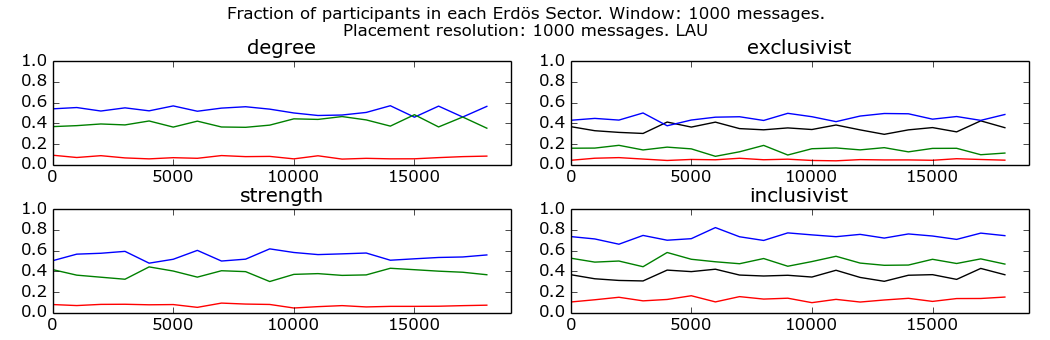
\includegraphics[width=\textwidth]{figs/InText-WLAU-S1000}
	\caption{Fractions of agents in each Erd\"os sector, where the fractions for hubs, intermediary and peripheral vertices are represented in red, green and blue, respectively. We used two simple criteria, namely degree and strength, for the graphics on the left. For the graphics on the right we employed the Exclusivist and Inclusivist compound criteria, with black lines representing the fraction of vertices without class and with more than one class, respectively. See Section~\ref{si:frac} of Supporting Information for a collection of such timeline figures with all simple and compound criteria and metrics. Table~\ref{tab:secE}, also from Supporting Information, presents these fractions of agents in snapshots of networks from Facebook, Twitter and Participa.br.}
	\label{fig:sectIL}
\end{figure*}


\begin{table}[h]
	\caption{Distribution of activity among participants. The first column presents the percentage of messages sent by the most active participant. The column for the first quartile ($1Q$) shows the minimum percentage of participants responsible for at least 25\% of total messages. Similarly, the column for the first three quartiles $1-3Q$ gives the minimum percentage of participants responsible for 75\% of total messages. The last decile $-10D$ column brings the maximum percentage of participants responsible for 10\% of messages.}
	\begin{center}
		\begin{tabular}{ | l ||  c | c | c | c | }
			\hline
			list & hub & $ 1Q $ & $ 1-3Q $ & $-10D$ \\ \hline
			LAU & 2.78  & 1.19 (26.35\%)  & 13.12 (75.17\%)  & 67.32 (-10.02\%) \\\hline
LAD & 4.00  & 1.03 (26.64\%)  & 11.91 (75.18\%)  & 71.14 (-10.03\%) \\\hline
MET & 11.14  & 1.02 (34.07\%)  & 8.54 (75.64\%)  & 80.49 (-10.02\%) \\\hline
CPP & 14.41  & 0.29 (33.24\%)  & 4.18 (75.46\%)  & 83.65 (-10.04\%) \\\hline

		\end{tabular}
	\end{center}
	\label{autores}
\end{table}


\subsection{Stability of principal components and the prevalence of symmetry over clusterization for dispersion}\label{prevalence}
The topology was analyzed using standard, well-established metrics of centrality and clustering.
We also introduced symmetry metrics because of evidence of their importance in social contexts~\cite{newmanEvolving}.
The contribution of each metric to the variance is very similar for all the networks, and did not vary with time.
In applying PCA to the snapshots, the contribution of each metric to the principal components presents very small standard deviation. Table~\ref{tab:pcain} exemplifies the principal components formation with all the metrics considered for the MET email list. Similar results are presented in Section~\ref{si:pcat} of the Supporting Information for the other lists, with separate consideration of strategic combinations of metrics.

\begin{table}[!h]
	\caption{Loadings for the 14 metrics into the principal components for the MET list, $ws=1000$ messages in 20 disjoint positioning. The clustering coefficient (cc) appears as the first metric in the Table, followed by 7 centrality metrics and 6 symmetry-related metrics. Note that the centrality measurements, including degrees, strength and betweenness centrality, are the most important contributors for the first principal component, while the second component is dominated by symmetry metrics. The clustering coefficient is only relevant for the third principal component. The three components have in average 80\% of the variance.}
		\footnotesize
		\begin{center}
\begin{tabular}{| l | c | c | c | c | c | c |}\cline{2-7}
\multicolumn{1}{c|}{} & \multicolumn{2}{c|}{PC1}          & \multicolumn{2}{c|}{PC2} & \multicolumn{2}{c|}{PC3}  \\\cline{2-7}\multicolumn{1}{c|}{} & $\mu$            & $\sigma$ & $\mu$         & $\sigma$ & $\mu$ & $\sigma$  \\\hline
$cc$ & 0.89  & 0.59  & 1.93  & 1.33  & 21.22  & 2.97 \\\hline
$s$ & 11.71  & 0.57  & 2.97  & 0.82  & 2.45  & 0.72 \\
$s^{in}$ & 11.68  & 0.58  & 2.37  & 0.91  & 3.08  & 0.78 \\
$s^{out}$ & 11.49  & 0.61  & 3.63  & 0.79  & 1.61  & 0.88 \\
$k$ & 11.93  & 0.54  & 2.58  & 0.70  & 0.52  & 0.44 \\
$k^{in}$ & 11.93  & 0.52  & 1.19  & 0.88  & 1.41  & 0.71 \\
$k^{out}$ & 11.57  & 0.61  & 4.34  & 0.70  & 0.98  & 0.66 \\
$bt$ & 11.37  & 0.55  & 2.44  & 0.84  & 1.37  & 0.77 \\\hline
$asy$ & 3.14  & 0.98  & 18.52  & 1.97  & 2.46  & 1.69 \\
$\mu^{asy}$ & 3.32  & 0.99  & 18.23  & 2.01  & 2.80  & 1.82 \\
$\sigma^{asy}$ & 4.91  & 0.59  & 2.44  & 1.47  & 26.84  & 3.06 \\
$dis$ & 2.94  & 0.88  & 18.50  & 1.92  & 3.06  & 1.98 \\
$\mu^{dis}$ & 2.55  & 0.89  & 18.12  & 1.85  & 1.57  & 1.32 \\
$\sigma^{dis}$ & 0.57  & 0.33  & 2.74  & 1.63  & 30.61  & 2.66 \\\hline\hline
$\lambda$ & 49.56  & 1.16  & 27.14  & 0.54  & 13.25  & 0.95 \\
\hline\end{tabular}
\end{center}

		\label{tab:pcain}
	\end{table}

The first principal component is an average of centrality metrics: degrees, strengths and betweenness centrality. Therefore, all of these centrality measurements are equally important for characterizing the networks. On one hand, the relevance of all centrality metrics is not surprising since they may be highly correlated. The degree and strength, for instance, are highly correlated, with Spearman correlation coefficient $\in [0.95,1]$ and Pearson coefficient $\in [0.85,1)$ for $ws>1000$. On the other hand, each of these metrics is related to a different participation characteristic, and their equal relevance is noticeable.
The clustering coefficient is presented in almost perfect orthogonality to centrality metrics.
\begin{figure*} 
	\centering
	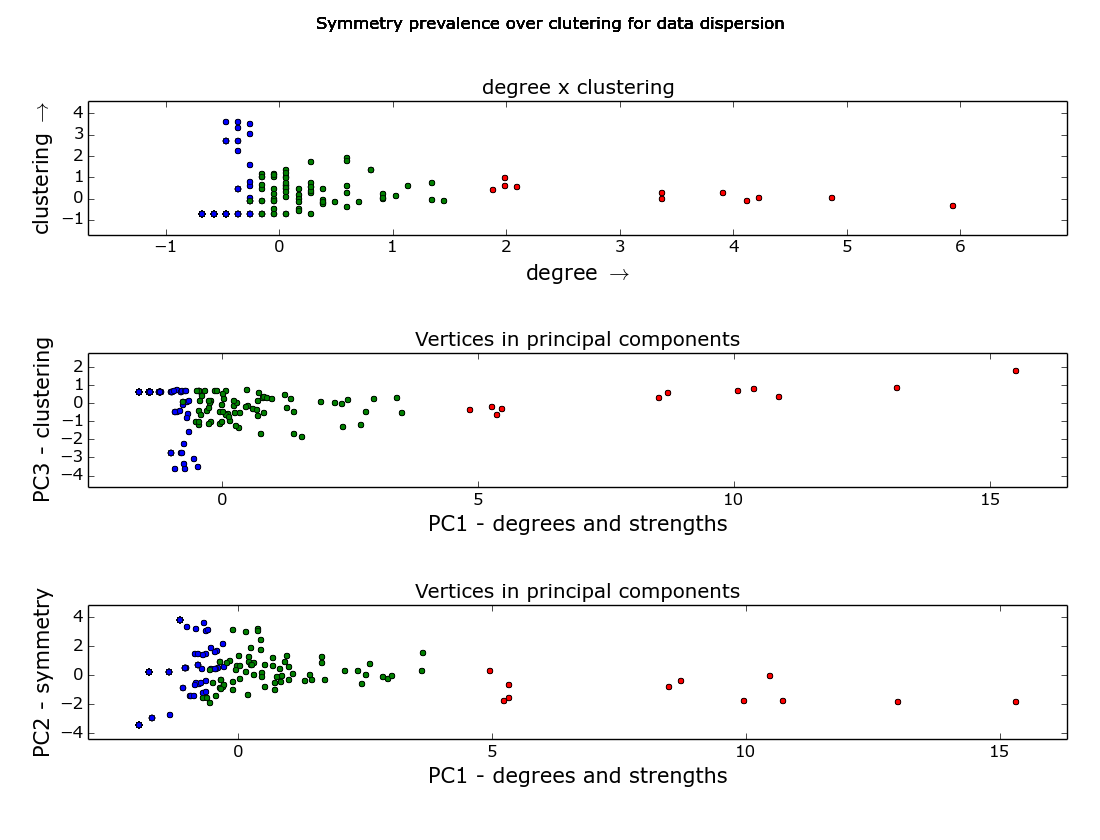
\includegraphics[width=.6\textwidth,height=10cm]{figs/im13PCAPLOT_}
	\caption{The first plot shows degree versus clustering coefficient. This typical pattern is well known, since high clustering is more incident in vertices with lower degrees. The second plot is analogous but the first component is an average of centrality metrics. The second component remains related to the clustering coefficient. The third plot exhibits the greater dispersion in the symmetry-related second component. In this case, the clustering coefficient is only relevant for the third component. This greater dispersion suggests that symmetry-related metrics are more powerful for characterizing interaction networks than the clustering coefficient, especially for hubs and intermediary vertices.
	This figure was obtained with a snapshot of the LAU list in a window size of $ws = 1000$ messages. Similar structures were observed in all window sizes $ws\;\in\;[500,10000]$ and for networks of other email lists, which points to a common relationship between the metrics of degrees, strengths and betweenness centrality, the symmetry-related metrics and clustering coefficient.}
	\label{fig:sym}
\end{figure*}

Dispersion was more prevalent in symmetry-related metrics than for the clustering coefficient, as indicated in Table~\ref{tab:pcain}. This is also illustrated in Figure~\ref{fig:sym}, where each vertex is colored according to the sector they belong to. As expected, peripheral vertices have very low values in the first component (centrality related) and greater dispersion in the third component (clustering related).
The PCA plot in the third system of Figure~\ref{fig:sym}, where all metrics are considered, reflects the relevance of the symmetry-related metrics for the variance.
We conclude that the latter metrics can be more meaningful in characterizing interaction networks (and their participants) than the clustering coefficient, especially for hubs and intermediary vertices.

The relative importance of the topological metrics was also observed for the additional 12 networks from Facebook, Twitter and Participa.br. With the exception of two of these networks, the overall behavior was maintained in that centrality measurements were found to be the most relevant to explain network topology, followed by symmetry-related metrics and then clustering coefficient. The results are given in Tables~\ref{tab:pcaE1F},~\ref{tab:pcaE1I},~\ref{tab:pcaE2},~\ref{tab:pcaE3} of the Supporting Information. There are larger differences between two of these networks than between two (GMANE) email networks, as the latter were much more regular.

\subsection{Types from Erd\"os sectors}\label{sec:pty}
A sector to which a vertex belongs can be regarded as yielding a type to the corresponding participant.
Assigning a type to a participant inevitably raises an important question regarding the possible stigmatization. 
We take the view that the participation typology inherent in the Erd\"os sectors is not stigmatizing because the type of an individual changes constantly~\cite{adorno}. 
That is to say, an individual is a hub in a number of networks and peripheral in other networks, and even within a network he/she probably changes type along time. 
Indeed, we did observe often transitions of participants from one sector to another.
The typology proposed here bridges exact and human sciences and may be enriched with concepts from other typologies, such as Meyer-Briggs, Pavlov or the authoritarian types of the F-Scale~\cite{adorno}.

We analyzed the time evolution of the networks using visualization tools developed for this research~\cite{rcText,versinus} and inspected the raw data to infer the main characteristics of each type. Our main observations may be summarized as follows:
\begin{itemize}
	\item Core hubs usually have intermittent activity. Very stable activity was found on MET hubs, which is consistent with the literature where greater stability occurs in smaller communities~\cite{barabasiEvo}.
	\item Typically, the activity of hubs is trivial: they interact as much as possible, in every occasion with everyone. The activity of peripheral vertices also follows a simple pattern: they interact very rarely, in very few occasions. Therefore, intermediary vertices seem responsible for the network structure. Intermediary vertices may exhibit preferential communication to peripheral, intermediary, or hub vertices; can be marked by stable communication partners; can involve stable or intermittent patterns of activity.
	\item Some of the most active participants receive many responses with relative few messages sent, and rarely are top hubs. These seem as authorities and contrast with participants that respond much more than receive responses.
	\item The most obvious community structure, as observed by a high clustering coefficient, is found only in peripheral and intermediary sectors.
\end{itemize}

With regard to the networks as the whole objects of analysis,
we were able to observe a negative correlation between the number of threads and the number of participants.
When the number of participants exceeds a threshold,
the number of threads displays a positive correlation with the number of participants.
This finding is illustrated in Figure~\ref{fig:nmgamma3d} and can also be observed in Table~\ref{tab:genLists}.
Obviously, network types can be derived from such results, which was not attempted here but 
left for the reader and future work. 

\begin{figure}
   \centering
        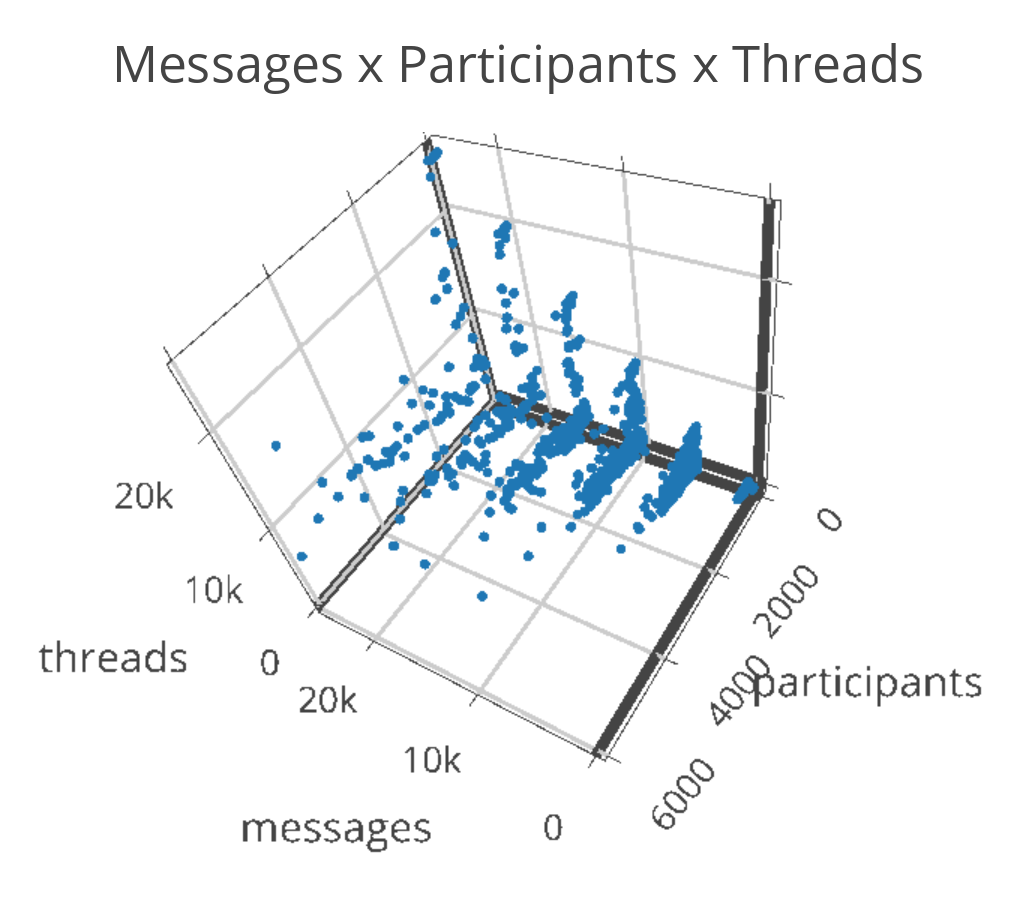
\includegraphics[width=\columnwidth]{figs/mpgamma____________}
	\caption{A scatter plot of messages (M) versus participants (N) versus threads ($\Gamma$) for 140 email lists. Highest number of threads are found in lists with few participants. The correlation between $N$ and $\Gamma$ is negative for low values of $N$ but positive otherwise. This negative correlation between $N$ and $\Gamma$ can also be observed in Table~\ref{tab:genLists}. For $M=20000$ messages, positive correlation of $N$ and $\Gamma$ is present mostly above 1500 participants. All LAU, LAD, MET lists present smaller networks.}
	\label{fig:nmgamma3d}
\end{figure}



\section{Conclusions}\label{sec:conc}
The most important result from the analysis of time evolution of the four email lists is certainly the time-independence observed not only for the activity but also for the properties of the networks themselves.
For example, the relative fractions of participants classified as hubs, intermediary and peripheral vertices remained practically constant along time, and this applied to all the email lists studied.
Furthermore, the PCA analysis of the topological metrics characterizing the networks also indicated that the contribution of each metric did not vary in time.
Centrality metrics were found to be the most relevant to characterize the network topology, followed by symmetry-related metrics, which were more relevant, with respect to variance, than clustering. 

A systematic study of the activity of participants belonging to the three distinct Erd\"os sectors indicated simple patterns for hubs and peripheral vertices, while the network structure was governed by the intermediary vertices. These properties were shared by all email lists and were time-independent, being consistent with the literature. Moreover, both the distribution of Erd\"os sectors and the contribution from the metrics to the PCA were found to apply to networks from Facebook, Twitter and Participa.br. We may therefore consider the classification of agents into Erd\"os sectors as leading to a human typology which bridges between exact sciences, with objective procedures for the classification, and human sciences, where there is a legacy in the observation of human types. 


\begin{acknowledgments}
	Financial support was obtained from CNPq (140860/2013-4,
	project 870336/1997-5), United Nations Development Program (contract: 2013/000566; project BRA/12/018) and FAPESP. 
	The authors are grateful to the American Jewish Committee for maintaining an online copy of the Adorno book used on the epigraph~\cite{adorno}, to GMANE creators and maintainers, and to the communities of the email lists and other groups used in the analysis, and to the Brazilian Presidency of the Republic for keeping Participa.br code and data open.
	We are also grateful to developers and users of Python scientific tools.
\end{acknowledgments}


%%%%%%%%%%%%%%%%%%%%%%%%%%%%%%%%%%%%%%%
\appendix
\section*{APPENDIX: Data and scripts}\label{scripts}
Messages were downloaded from the GMANE public database~\cite{GMANEwikipedia}. Data annotated from Facebook and Twitter are in a public repository~\cite{fbtwData}. Data from Participa.br was used from the linked data/semantic web RDF triples reported in~\cite{opa} and available in~\cite{datahub}.
All routines necessary to achieve the results reported in this article, including all tables and figure of the Supporting Information, are available through a public domain Python package and an open Git repository~\cite{gmanePack}. Data from social networks used in this study were gathered and used within the Anthropological Physics principles~\cite{anPhy}.

%\nocite{*}
\bibliography{paper}% Produces the bibliography via BibTeX.

\end{document}
%
% ****** End of file aipsamp.tex ******



